\subsection{Analysis and Limitations}
\label{subsec:analysis_limitations}

\subsubsection{Comparison with the Closest Prior Work}
\label{subsec:vs_mambaofr}

MgfrOFR is built directly on top of MambaOFR~\cite{mao2025mambaofr}, so its contribution should be distinguished from the baseline backbone. We do not claim originality for bidirectional Mamba propagation, the degradation-aware prompt block, or the original reconstruction head. The contribution of this work is the reorganization and regularization of propagated features before reconstruction.

Compared with MambaOFR, MgfrOFR differs in four implementation-level aspects. First, the propagated feature is no longer treated as a single restoration carrier; MGFE exposes explicit coarse-to-fine branches. Second, these branches are summarized and fed back through channel-wise recalibration rather than used only for auxiliary supervision. Third, branch diversity is constrained by ranking correlation on temporal correspondences rather than by an identity-based objective from recognition tasks. Fourth, RATR is used only during training, so the deployment interface remains compatible with the baseline inference pipeline.

The symmetry-related claim is limited to representation balance. MgfrOFR does not model object-level geometric regularity and does not propose a general mathematical theory of symmetry. Instead, it studies whether coarse-to-fine restoration branches can remain balanced under asymmetric film degradation. MGFE separates evidence by restoration granularity, and RATR discourages redundant temporal-similarity rankings across branches.

\subsubsection{MGFE--RATR Synergy for Branch Balance}
\label{subsec:synergy}

The ablation study indicates that MGFE and RATR have different roles in the full model. RATR alone provides a stronger and more stable gain than MGFE recalibration alone (Table~\ref{tab:ablation}) because the RATR-only configuration still computes MGFE branch descriptors and uses them as multi-granularity ranking targets; only the channel-wise scale/shift feedback is disabled. MGFE creates the branch structure needed for coarse-to-fine feature balance, whereas RATR makes the branches more complementary by suppressing redundant temporal-ranking behavior.

The real-world results are consistent with this interpretation but do not prove content fidelity without ground truth. On the SRWOV real-world test set (Table~\ref{tab:realworld}), MgfrOFR achieves the best NIQE and BRISQUE and remains competitive on CLIP-IQA+, suggesting that the multi-granularity decomposition transfers useful restoration structure beyond the synthetic training distribution. Because these are no-reference metrics, the claim is limited to statistical naturalness and metric-based perceptual quality.

\subsubsection{Branch Balance Analysis}
\label{subsec:branch_analysis}

The branch analysis assesses whether the granularity branches remain complementary rather than becoming correlated copies of the same descriptor. We compute pairwise cosine similarity between branch descriptors on the SRWOV synthetic test set. This analysis directly supports the representation-balance claim: useful branches should remain comparable but not redundant.

The full model yields lower inter-branch similarity than the MGFE-only variant (Figures~\ref{fig:branch_similarity} and~\ref{fig:branch_error_map}). This supports the role of RATR as the mechanism that keeps granularity branches functionally distinct. The RATR-only variant remains closer to the full model than to MGFE-only, which further indicates that ranking diversity regularization suppresses collapse even before recalibration feedback is enabled.

Figure~\ref{fig:branch_similarity} illustrates this contrast for a representative frame. In the MGFE-only configuration, the off-diagonal similarities remain high, indicating that the branches encode nearly the same restoration evidence. In the full model, these off-diagonal values decrease markedly, especially for the fine-grained branch, showing a more differentiated branch geometry.

\begin{figure}[!t]
\centering
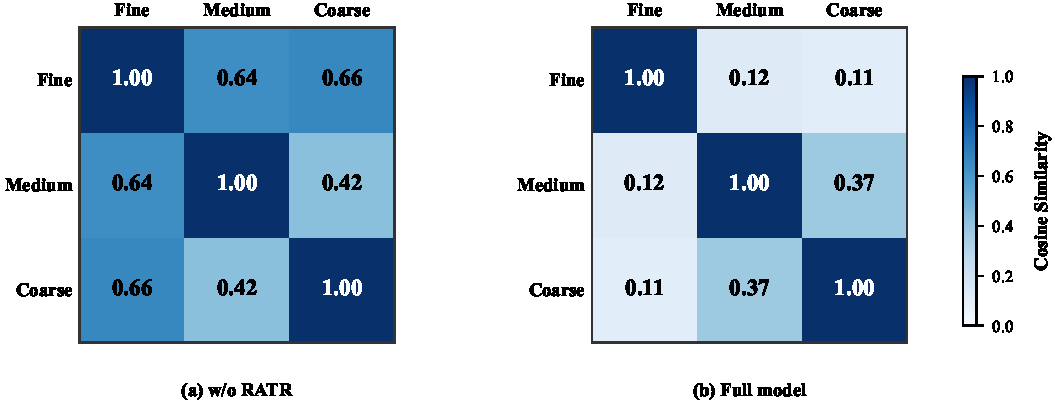
\includegraphics[width=0.84\textwidth]{figures/Fig9a_branch_similarity.pdf}
\caption{Branch balance analysis. Pairwise cosine similarity is compared between the MGFE-only configuration and the full MgfrOFR model. RATR reduces off-diagonal similarity from 0.42--0.66 to 0.11--0.37, confirming that ranking-aware regularization prevents granularity branches from collapsing into correlated descriptors.\label{fig:branch_similarity}}
\end{figure}

\begin{figure}[!t]
\centering
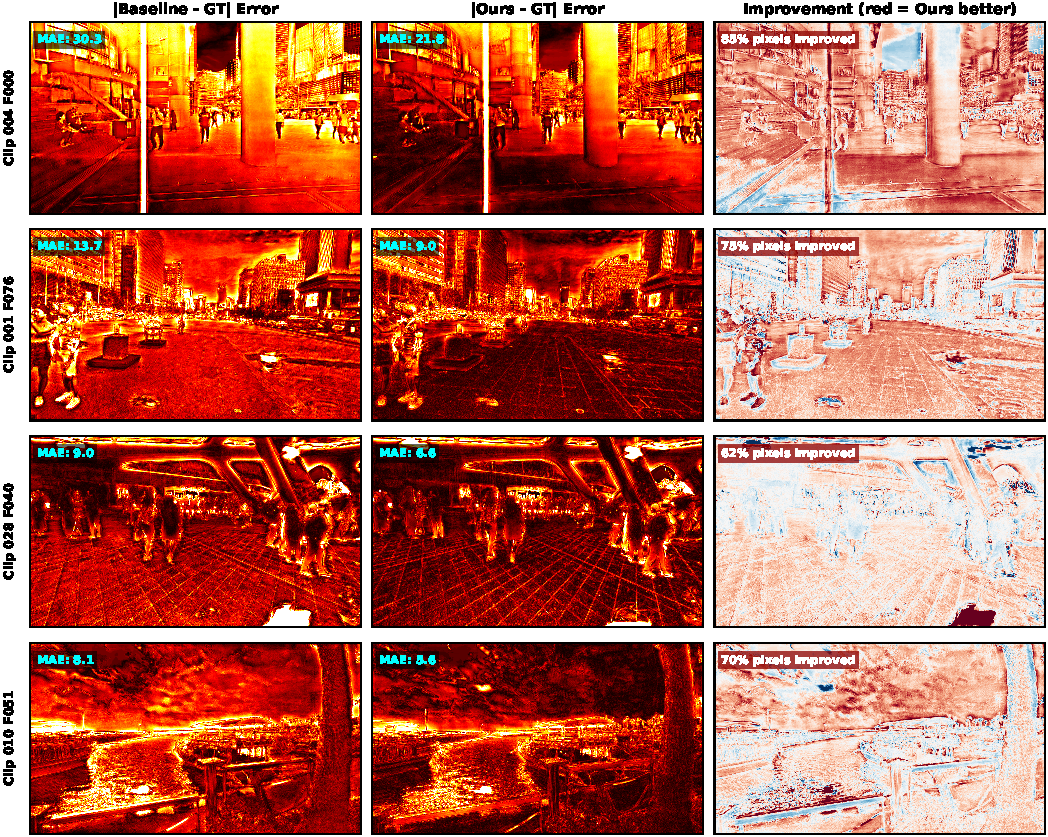
\includegraphics[width=0.98\textwidth]{figures/Fig9b_error_map.pdf}
\caption{Pixel-wise absolute-error comparison on four gate-selected synthetic frames. The left and middle columns compare $|$Baseline $-$ GT$|$ and $|$MgfrOFR $-$ GT$|$; the right column illustrates their difference, where red indicates regions in which MgfrOFR reduces the reconstruction error. The error maps demonstrate that lower branch correlation translates into spatially broader restoration gains rather than isolated local fixes.\label{fig:branch_error_map}}
\end{figure}

The inspected examples suggest a consistent specialization pattern. The fine-grained branch is most sensitive to localized defects such as scratches and pixel-level noise; the coarse branch emphasizes broader structural corruption such as blotches and cracks; and the medium branch occupies an intermediate role. This behavior is consistent with progressive token fusion, where fewer surviving tokens aggregate over wider spatial support. The pixel-domain error maps in Figure~\ref{fig:branch_error_map} further indicate that branch decorrelation corresponds to broader restoration gains rather than isolated local fixes.

\subsubsection{When Does MgfrOFR Struggle?}
\label{subsec:failure}

MgfrOFR's advantage is not uniform across all degradation conditions. The ablation study (Table~\ref{tab:ablation}) shows that MGFE alone degrades perceptual quality, and the visual ablations suggest that the full model is most useful when heterogeneous degradation is present, such as structural damage co-occurring with fine scratches in the same frame. On clips dominated by a single degradation type, such as uniform flicker without spatial damage, the multi-granularity decomposition can add representational overhead without proportional benefit, and the baseline or RATR-only variant may match the full model's fidelity.

The real-world CLIP-IQA+ result highlights a trade-off between naturalness and enhancement-oriented perceptual quality. MgfrOFR's CLIP-IQA+ (0.4368) ranks second to OldPhoto (0.4503), while MgfrOFR achieves the best NIQE (5.06) and BRISQUE (18.70). This pattern reflects that different no-reference metrics measure distinct aspects of restoration quality. CLIP-IQA+ is trained on human quality annotations that correlate with sharp textures and high-contrast details~\cite{wang2023clipiqa}, favoring methods such as OldPhoto that enhance perceptual sharpness through learned global priors. NIQE and BRISQUE instead measure statistical deviation from natural image distributions and penalize artifacts introduced by texture hallucination. MgfrOFR's granularity-based recalibration operates conservatively on the propagated feature stream, which appears to preserve statistical naturalness while providing less texture enhancement than OldPhoto. For archival restoration, NIQE/BRISQUE may be more relevant proxies when content fidelity is prioritized, but a human study is needed to validate that preference.

\subsubsection{Limitations, Threats to Validity, and Future Work}
\label{subsec:limitations}

\paragraph{Threats to Validity.}
Five threats affect the interpretation of the results. \textbf{Dataset threat}: all training uses synthetic degradation applied to REDS clips, which introduces a synthetic-to-real domain gap and may limit generalization to archival footage with correlated degradation chains not modeled by the pipeline. \textbf{Metric threat}: evaluation relies on PSNR/SSIM for pixel fidelity and no-reference metrics for real-world assessment; these metrics emphasize different aspects of quality and may not fully align with human perceptual judgments, especially for perceptual metrics where inter-clip variance prevents statistical significance at $N{=}30$. \textbf{Human-evaluation threat}: the study does not include an expert reader study with film-restoration practitioners or archivists, so the practical value of improvements on authentic footage is inferred from proxy metrics and qualitative inspection. \textbf{Baseline threat}: three baselines (VRT, RVRT, ShiftNet) required adaptation from video restoration to OFR-specific degradation, which preserves their architectures but may not reflect their optimal performance under a different training regime. \textbf{Synthetic-to-real threat}: the real-world evaluation lacks ground truth, so improvements in NIQE/BRISQUE reflect statistical naturalness rather than verified content fidelity, and the absence of external validation on additional datasets weakens the generalization claim.

\paragraph{Limitations and Future Work.}
RATR adds a training-time cost because it requires branch-wise similarity matrices over the batch-time descriptor set $\bar{N}=BT$. Its dominant cost therefore grows approximately quadratically in $\bar{N}$. In our setting ($B{=}4$, $T{=}7$, $G{=}3$), the total overhead of MGFE and RATR is 0.5\,GB (7.0 vs.\ 6.5\,GB; Table~\ref{tab:complexity}); however, longer clips or larger effective batch-time products would make this quadratic term more pronounced. Gradient checkpointing or selective ranking construction, such as sampling a subset of anchors per iteration, will be needed for larger training settings. The second limitation is the synthetic-to-real domain gap caused by REDS-based training degradation. Although the real-world NIQE/BRISQUE results are encouraging, authentic archival footage can contain correlated degradation chains that synthetic pipelines do not model. The third limitation is evaluation scope: validation is limited to SRWOV, and additional archival datasets plus human evaluation would strengthen the generalization claim.

Promising extensions include adaptive branch activation conditioned on degradation severity, frequency-aware branch specialization that assigns structural recovery and texture restoration to dedicated branches, and joint OFR--colorization frameworks for archival digitization and cultural heritage restoration workflows~\cite{kokaram2004missing}.
